\chapter{Complementary information}
\label{app:complement}

Additional material. For example long mathematical derivations could be
given in the appendix. Or you could include part of your code that is
needed in printed form. You can add several Appendices to your thesis (as
you can include several chapters in the main part of your work).

\section{Including \Rp code with verbatim}
A simple (rather too simple, see~\ref{App:listings}) way to include code or
{\it R} output is to use 
\texttt{verbatim}. It just prints the text however it is (including all
spaces, ``strange'' symbols,...) in a slightly different font.
\begin{verbatim}
## loading packages
library(RBGL)
library(Rgraphviz)
library(boot)

## global variables
X_MAX <- 150

   This allows me to put as many s  p a   c es   as I want.
I can also use \ and ` and & and all the rest that is usually only 
accepted in the math mode.

I can also make as 
                  many 
             line 
    breaks as 
I want... and
             where I want. 
\end{verbatim}

\section{Data Processing Code}\label{app:proccode}
However, it is much nicer to use the \emph{listings} package to include \Rp
code in your report. It allows you to number the lines, color the comments
differently than the code, and so on.

\lstinputlisting{Pictures/DataProcess.R}


\section{Jury Sunshine Irregularities} \label{app:irregs}

\begin{table}[h]
  \caption[Jury Sunshine Irregularities]{Jury sunshine data irregularities noted in data flattening}
  \centering
  \begin{tabularx}{\textwidth}{|c|X|} \hline
    Charges without trial (ACISID) & 08CRS50940, 08CRS52888, 09CRS000305, 09CRS1106, 09CRS50752, 10CR52031, 10CRS051975,
    10CRS1215, 10CRS397, 10CRS51388, 10CRS51610, 10CRS52410, 11CRS051642, 11CRS051795, 11CRS1577, 11CRS1745, 11CRS1783,
    11CRS51204, 11CRS51895, 11CRS52470, 08CRS54836, 08CRS50113 \\ \hline 
    Prosecutors without trials (IDs) & 1-000, 11B-000, 12-000, 14-000, 15B-000, 16A-000,
                     16B-000, 17A-000, 17B-000, 19A-000, 19B-000,
                     20A-000, 20B-000, 21-000, 22A-000, 22B-000,
                     24-000, 25-000, 27A-000, 27B-000, 28-000,
                                       29A-000, 29B-000, 30-000, 6-000, 9-000 \\ \hline
    Trial missing charge (ID) & 710-01 \\ \hline
  \end{tabularx}
\end{table}

\section{Jury Sunshine Charge Classification} \label{app:charge}

\begin{figure}[!h]
  \centering
  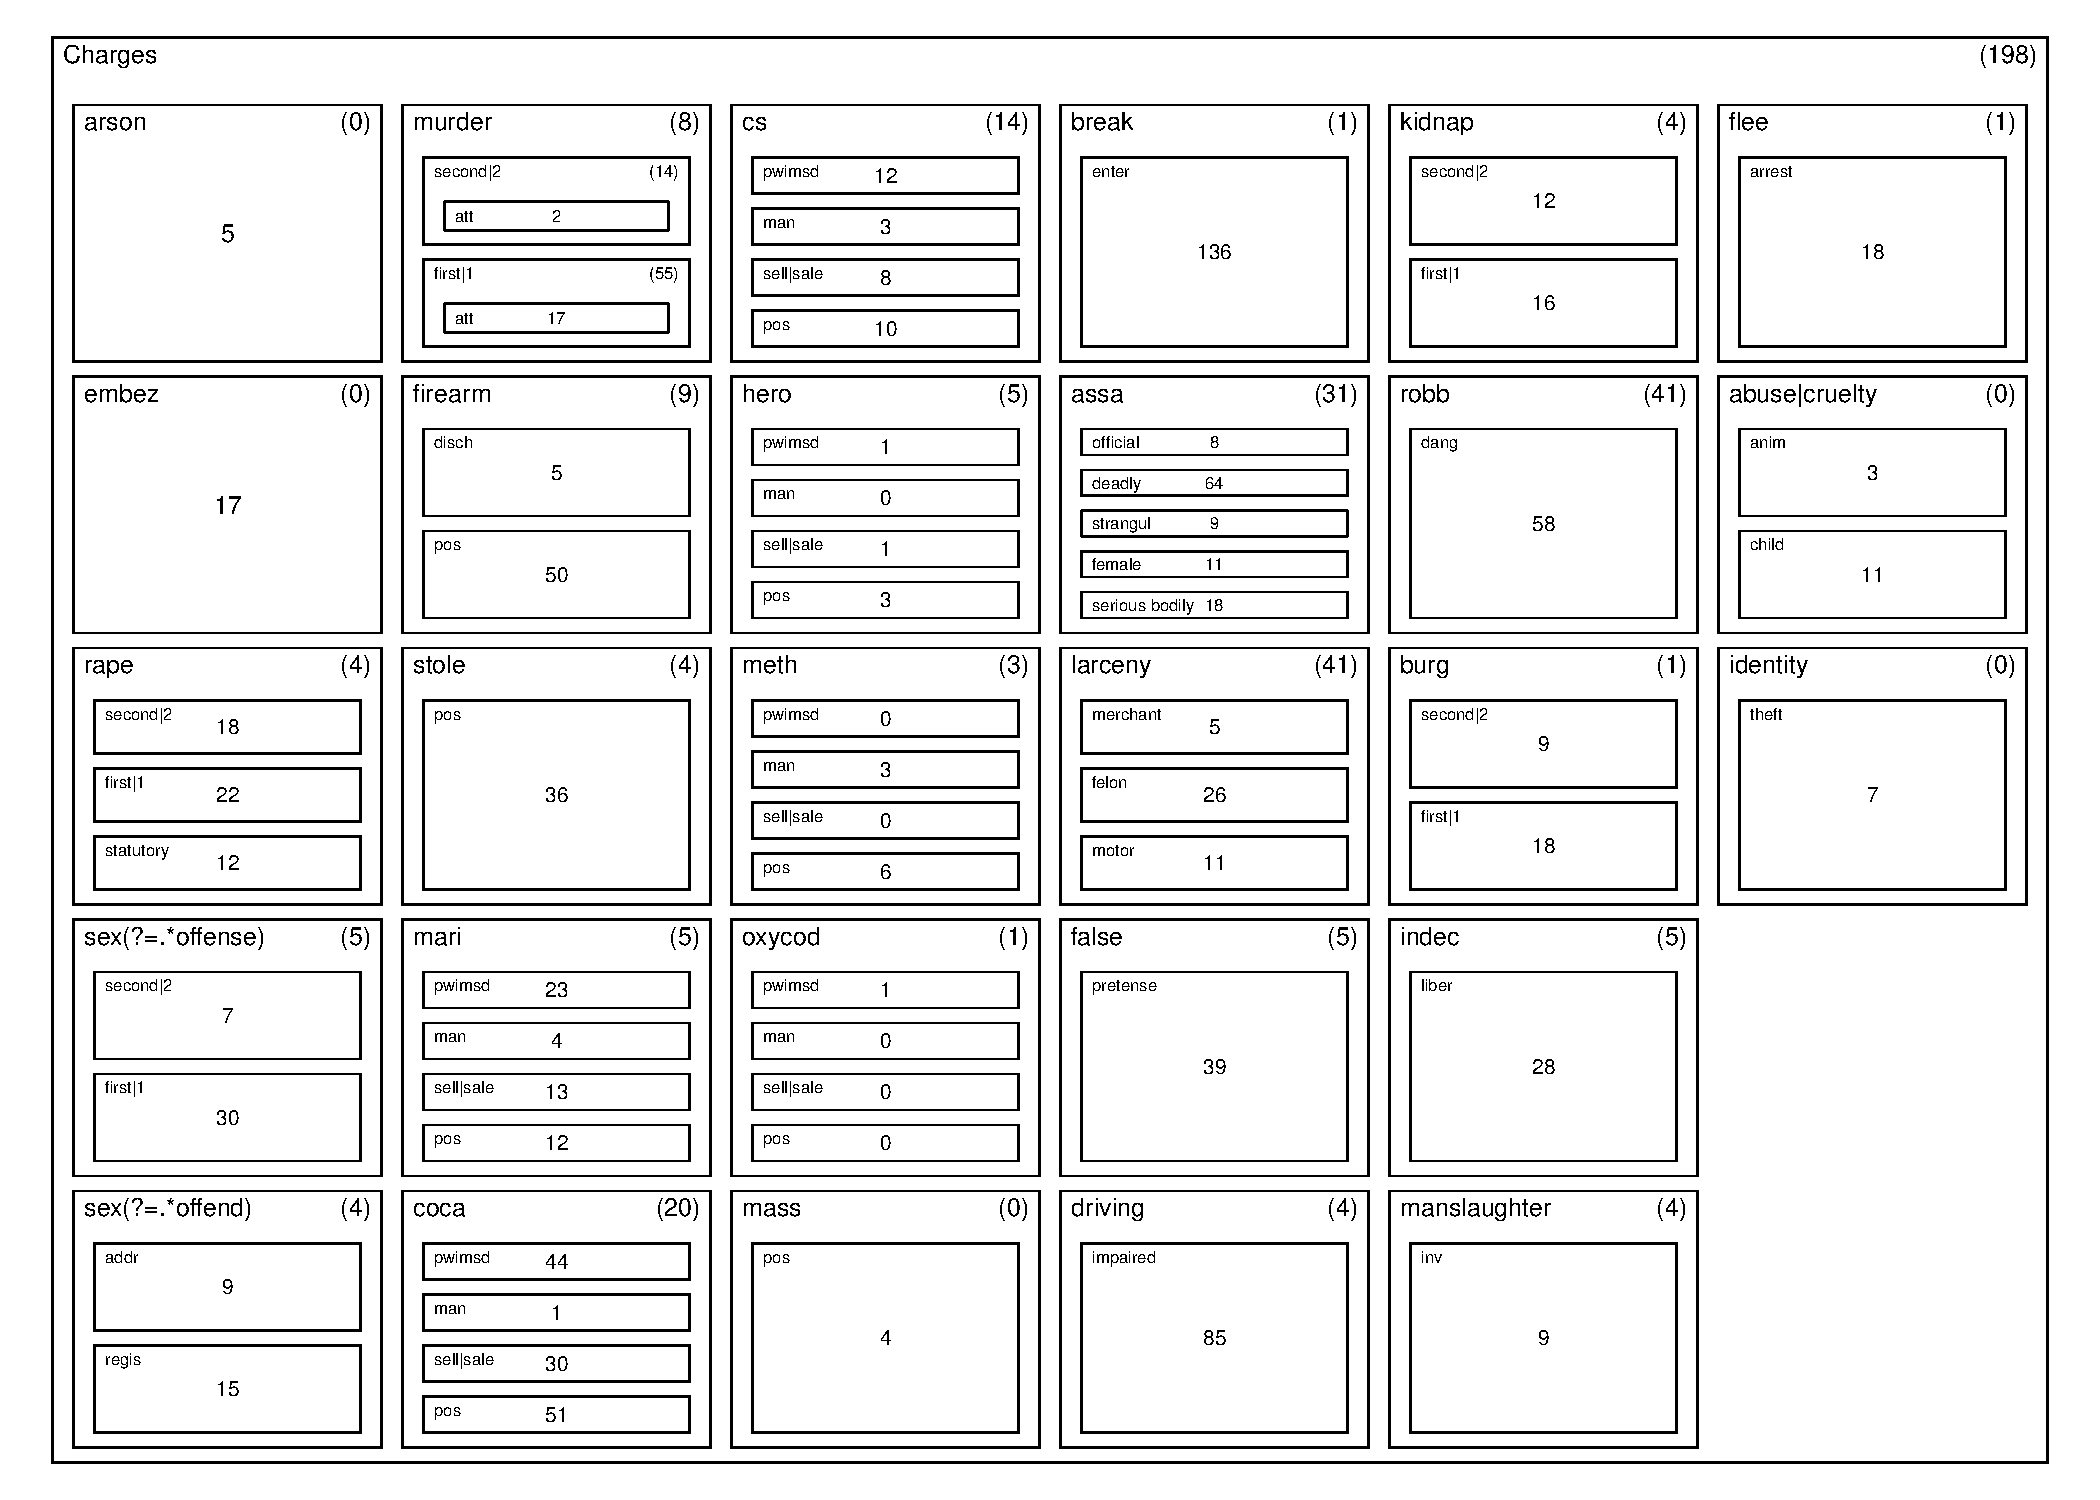
\includegraphics[angle=90, origin=c, width=1\textwidth]{ChargeDiagram}
  \caption[Regular expression charge tree visualized]{The regular expression charge tree arranged by hierarchy with counts
    provided. The counts in brackets indicate the counts of charges which could not be classified to a lower level of the
    hierarchy}
  \label{fig:chargetree}
\end{figure}

\section{Analysis Code} \label{app:analysis}

\lstinputlisting{Pictures/AnalysisScript.R}

\section{Using Sweave to include \Rp code (and more) in your report}
The easiest (and most elegant) way to include \Rp code and its output (and
have all your figures up to date with your report) is to use Sweave. You
can find an introduction Sweave in \texttt{/u/sfs/StatSoftDoc/Sweave/Sweave-tutorial.pdf}.

%%% Local Variables: 
%%% mode: latex
%%% TeX-master: "MasterThesisSfS"
%%% End: 
